% mainfile:main.tex
% revised by dnolivieri

\chapter[GNOME 3.0 for application developers]{GNOME 3.0 for application developers\cite{website:gnome-3-0-for-application-developers}}\label{GNOME3AppDevs}

This is specifically for \emph{gedit} but it applies to other \GNOME applications, as most of them had to pass the storm that is \GNOME 3.0.

gedit is almost solely being developed by volunteers (it has been shown that little to none of the contributions are from financed developers). This is of course true for many open source projects. gedit appears to be  simple application, however in reality it is quite extensive and complicated.

The normal development cycles are relatively uneventful. A small set of new features are introduced, some bug fixes are provided, etc. Also, 
a stable current HEAD of development is always ensured to be ``stable''.
gedit developers have always used current HEAD in a production environment, which refers to versions that receive a large amount of testing, 
since it is an application that many users utilize every day. 



Traditionally, gedit has not been an early adopter of new technologies, opting 
to wait for the testing of other applications which helped this level of stability.
This situation changed with GNOME 3.0.  The developer community decided to try to adopt changes as early as possible in the development cycle, 
so that gedit would be ready to be shipped with all changes incorporated. This meant however, among other things, the following:
\begin{itemize}
  \item A lot of work to port from ``old'' technologies (gconf – gsettings, pygtk – pygi).
  \item A lot of time has been invested on trying to get the jhbuild environment ready for developing.
  \item gedit is continuously broken due to API changes or broken dependencies.
  \item No real testing because it is unusable in a production environment.
  \item Regressions are almost inevitable.
  \item No real change for end users!
\end{itemize}

Of course, while the advantage of this new philosophy of adopting new technologies early in the development cycle is the advantages are clear, 
it has been a stress on the small team of gedit developers.   In order to illustrate the impact of this, here are some statistics related to 
our development cycles.

\addfigure[width=0.70\textwidth]{./images/gedit-development}{gedit Development}{fig:geditDevelopment}

On this plot can be seen the sum of all added and removed lines (excluding translations) over all commits in a particular development cycle. As can be appreciated, a significant increase of activity in this cycle it is noted. Of course, not all of this can be attributed to \GNOME 3.0, but there is an undeniable effect.   Zooming in the last two development cycle the work made by each developer on this team can be seen.

\begin{figure}[H]
  \begin{minipage}[b]{0.5\linewidth}
    \centering
    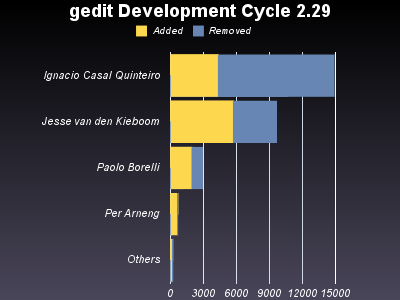
\includegraphics[scale=0.45]{./images/gedit-development-2-29}
    \caption{gedit development 2.29}
  \end{minipage}
  \hspace{0.5cm}
  \begin{minipage}[b]{0.5\linewidth}
    \centering
    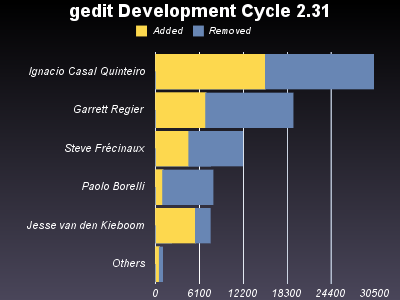
\includegraphics[scale=0.45]{./images/gedit-development-2-31}
    \caption{gedit development 2.31}
  \end{minipage}
\end{figure}

It is important to note that this cycle has been particularly difficult for application developers, especially those that try to adopt early, 
so that they are actually ready by the time GNOME 3.0 is ready for release.   And then to think, for the end user, there will be basically no 
change at all.

